\chapter{البطاريات وخلايا الوقود والتحليل الكهربائي}\label{ch:b2:batteries-electrolysis}

كل كيلوغرام من الألومنيوم يُستخلص من خامه يتطلب نحو \qty{13}{kW.h} من
الكهرباء؛ أما صهر كيلوغرام من الخردة فيتطلب، من حيث المبدأ،
\qty{0.3}{kW.h} التي ترفعه إلى درجة انصهاره وتصهره. والفرق
هو عمل صف طويل من خلايا \omterm{def:b2:batteries-electrolysis:electrolysis}{التحليل الكهربائي}، يمرر كل منها مئات
آلاف الأمبيرات في ملح منصهر تحت بضعة فولطات. والبطارية تعمل في
الاتجاه المعاكس: فتفاعل تلقائي هو الذي يدفع التيار. وبمنحنيات
شدة التيار--الجهد في \cref{ch:b2:current-potential-curves}، تُقرأ الحالتان
على المخطط نفسه، وكذلك قطعة زنك تذوب في حمض.
% ledger: hT:Al_l.933, aw:Al

\begin{recall}
\Cref{ch:b2:cell-thermodynamics}: $\Delta_r G = -nFE$، والشغل الأقصى، \omterm{def:b2:cell-thermodynamics:faraday}{وثابت
فاراداي}. \Cref{ch:b2:current-potential-curves}: منحنيات شدة التيار--الجهد،
والأنظمة السريعة والبطيئة، \omterm{def:b2:current-potential-curves:overpotential}{وفرط الجهد}، والتيارات الحدية، وجدارا
الماء. \Cref{ch:b2:ellingham}: لماذا لا يُستخلص الألومنيوم بالكربون. والمجلد
المدرسي: \omterm{def:b2:batteries-electrolysis:electrolysis}{التحليل الكهربائي}، والمراكم.
\end{recall}

\begin{omfigure}
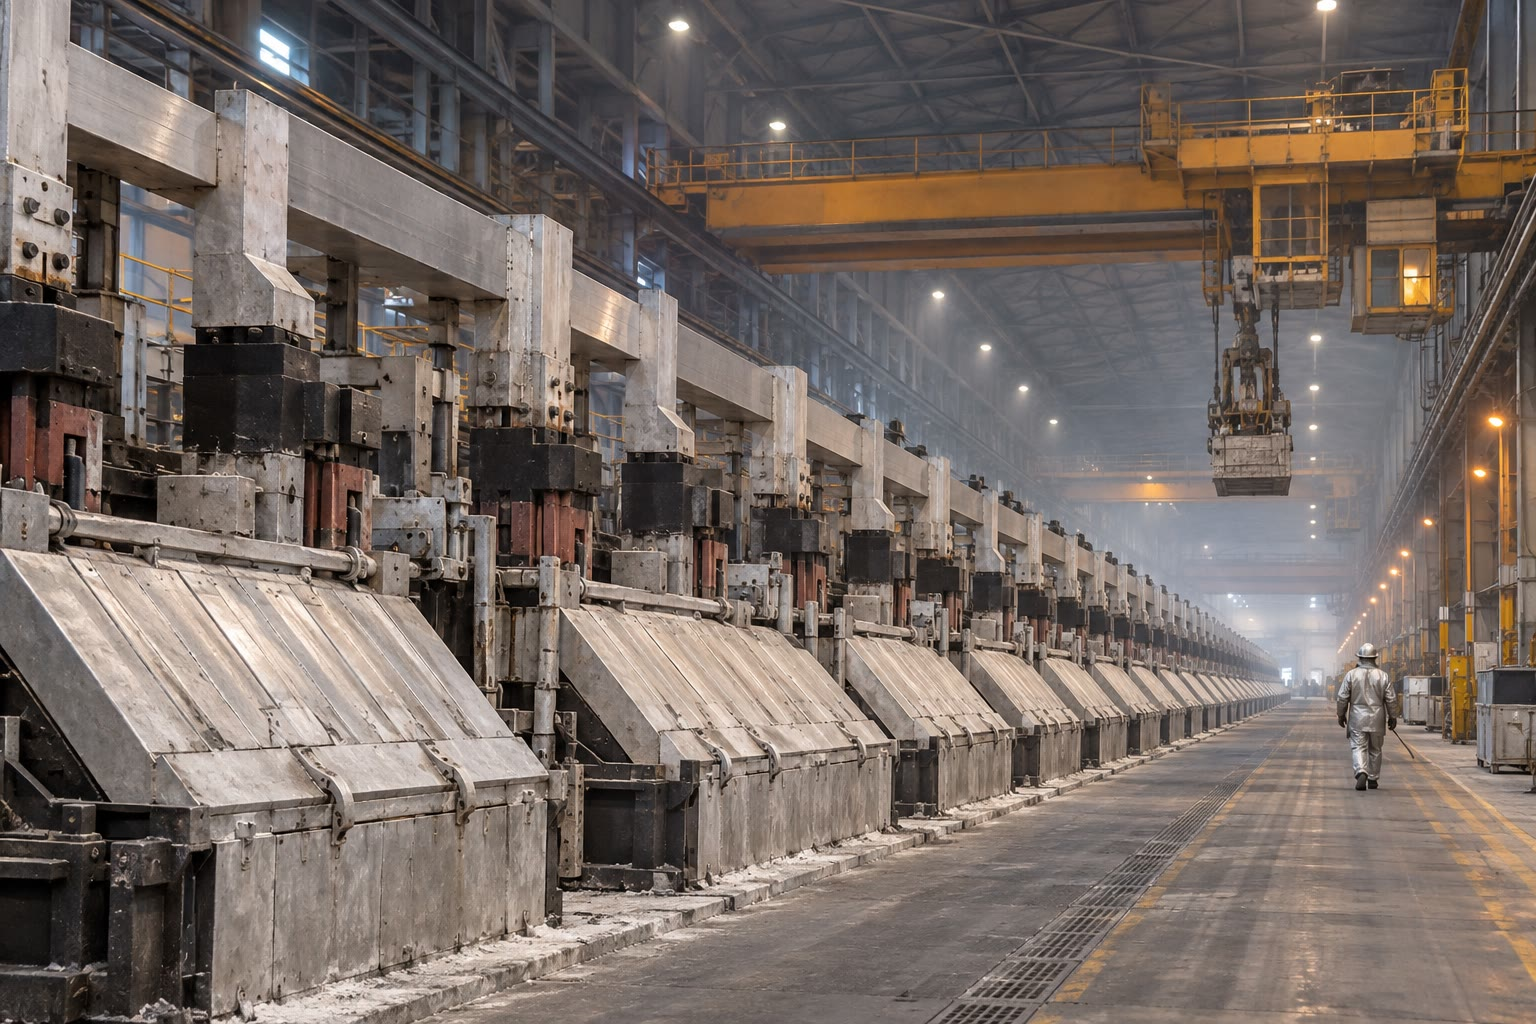
\includegraphics[width=0.62\linewidth]{images/book3/ai/b2-11-potroom.jpg}

{\small قاعة الخلايا في مصهر ألومنيوم: صف من خلايا \omterm{def:b2:batteries-electrolysis:electrolysis}{التحليل الكهربائي}،
طوله مئات الخلايا، موصولة على التوالي؛ وتغيّر الرافعة العلوية المصاعد
الكربونية كلما احترقت.}
\end{omfigure}

\section{التفاعلات التلقائية مقروءة على المنحنيات}

\begin{definition}[الجهد المختلط]\label{def:b2:batteries-electrolysis:mixed-potential}
\emph{الجهد المختلط}\index{جهد مختلط} لقطب تتفاعل عليه
مزدوجتان مختلفتان، تتأكسد إحداهما وتُختزل الأخرى، هو الجهد الذي
يأخذه حين لا يمر أي تيار صافٍ: فيكون \omterm{def:b2:current-potential-curves:ie-curve}{التيار المصعدي} لإحدى المزدوجتين
مساويًا ومعاكسًا \omterm{def:b2:current-potential-curves:ie-curve}{للتيار المهبطي} للأخرى.
\end{definition}

\begin{proposition}[فلز في محلول]\label{prop:b2:batteries-electrolysis:mixed}
يستقر فلز مغمور في محلول قادر على أكسدته عند الجهد
$E_m$ حيث $i_a(E_m) = -i_c(E_m)$، فيوازن \omterm{def:b2:current-potential-curves:ie-curve}{التيار المصعدي} لأكسدة الفلز
\omterm{def:b2:current-potential-curves:ie-curve}{التيار المهبطي} لاختزال المؤكسد؛ ويذوب
الفلز بالسرعة $i_a(E_m)/(nF)$.
\end{proposition}

\begin{proof}
قطعة الفلز المعزولة لا تحمل أي تيار صافٍ. ويجري نصفا التفاعل كلاهما
على سطحها عند الجهد نفسه، فيكون مجموع تياريهما، المقروءين على منحنييهما
عند ذلك الجهد، معدومًا. وحسب \cref{prop:b2:current-potential-curves:current-rate}،
يعطي \omterm{def:b2:current-potential-curves:ie-curve}{التيار المصعدي} سرعة الأكسدة.
\end{proof}

\begin{omfigure}
\begin{tikzpicture}
\begin{axis}[omie, width=0.82\linewidth, height=6cm, xmin=-1.1, xmax=-0.3,
  ymin=-3, ymax=3, xlabel={\babelsublr{$E$ (V)}}, ylabel={$i$}, clip=true, clip mode=individual,
  axis y line=left]
\addplot[omanodic] table[x=E, y=i] {figdata/out/bachelor-2-ie-curves-f-Zn.dat};
\addplot[omcathodic] table[x=E, y=i] {figdata/out/bachelor-2-ie-curves-f-HZn.dat};
\addplot[omcathodic, dashed] table[x=E, y=i] {figdata/out/bachelor-2-ie-curves-f-HCu.dat};
\draw[densely dotted] (axis cs:-0.820,-0.148) -- (axis cs:-0.820,0.148);
\draw[densely dotted] (axis cs:-0.737,-2.38) -- (axis cs:-0.737,2.38);
\fill (axis cs:-0.820,0.148) circle (1.3pt); \fill (axis cs:-0.737,2.38) circle (1.3pt);
\node[font=\scriptsize, anchor=south east] at (axis cs:-0.825,0.2) {الزنك وحده};
\node[font=\scriptsize, anchor=west] at (axis cs:-0.73,2.38) {الزنك ملامسًا للنحاس};
\node[font=\scriptsize, omThm, anchor=west] at (axis cs:-0.70,1.2) {\babelsublr{\ce{Zn} $\to$ \ce{Zn^2+}}};
\node[font=\scriptsize, omDef, anchor=north west, align=left] at (axis cs:-0.87,-0.5) {\babelsublr{\ce{H+} $\to$ \ce{H2}}\\ على الزنك};
\node[font=\scriptsize, omDef, anchor=north west] at (axis cs:-0.66,-1.7) {على النحاس};
\end{axis}
\end{tikzpicture}

{\small الزنك في الحمض (منحنيات نموذجية، وأيونات الزنك مخففة؛ والجهود من
$-1.1$ إلى \qty{-0.3}{V}). يستقر الزنك وحده عند
\omterm{def:b2:batteries-electrolysis:mixed-potential}{الجهد المختلط} الذي توازن فيه أكسدته الاختزالَ البطيء لأيونات
\ce{H+} على الزنك: تيار صغير، وذوبان بطيء. أما ملامسًا للنحاس، الذي يكون
اختزال \ce{H+} عليه أقل بطئًا، فينتقل التوازن إلى جهد أعلى
وتيار أكبر بأكثر من عشر مرات: فيذوب الزنك بسرعة، وتتصاعد فقاعات الهيدروجين
على النحاس.}
\end{omfigure}

القراءة نفسها تفسر التآكل (\cref{ch:b2:corrosion}): فسرعة تآكل
الفلز هي التيار عند جهده المختلط.

\section{الخلايا المعطية للتيار}

\begin{definition}[البطاريات]\label{def:b2:batteries-electrolysis:battery}
\emph{الخلية الأولية}\index{خلية أولية} خلية كهروكيميائية تُستعمل
مرة واحدة، حتى تنفد كواشفها. و\emph{المركم}\index{مركم}
خلية يمكن إعادة شحنها بإجبار تيار على المرور فيها في
الاتجاه المعاكس، وهو ما يعكس تفاعلها. و\emph{الطاقة
النوعية}\index{طاقة نوعية} للخلية هي الطاقة الكهربائية التي تعطيها
لكل وحدة كتلة، وتقاس عادة بوحدة \unit{W.h/kg}.
\end{definition}

\begin{proposition}[جهد خلية تعطي تيارًا]\label{prop:b2:batteries-electrolysis:delivering}
للخلية التي تعطي تيارًا $I$ جهد
\[
  U = E_+ - E_- - \eta_a - |\eta_c| - rI ,
\]
حيث $E_+$ و$E_-$ جهدا التوازن لقطبيها،
و$\eta_a > 0$ \omterm{def:b2:current-potential-curves:overpotential}{فرط جهد} الأكسدة عند القطب السالب،
و$\eta_c < 0$ \omterm{def:b2:current-potential-curves:overpotential}{فرط جهد} الاختزال عند القطب الموجب، و$r$ المقاومة
الداخلية (الإلكتروليت، والفاصل، والوصلات).
\end{proposition}

\begin{proof}
التيار نفسه $I$ مصعدي عند القطب السالب، الذي يُقرأ جهده
على منحناه المصعدي، $E_- + \eta_a$، ومهبطي عند القطب الموجب،
الذي جهده $E_+ + \eta_c$. وبينهما يعبر التيار
الإلكتروليت، حيث ينخفض الجهد بمقدار $rI$. ومنه $U = (E_+ + \eta_c) - (E_- +
\eta_a) - rI$.
\end{proof}

\begin{omfigure}
\begin{tikzpicture}
\begin{axis}[omie, width=0.82\linewidth, height=5.6cm, xmin=-1.2, xmax=0.8,
  ymin=-2, ymax=2, xlabel={\babelsublr{$E$ (V)}}, ylabel={$i$}, clip=true, clip mode=individual]
\addplot[omanodic] table[x=E, y=i] {figdata/out/bachelor-2-ie-curves-h-neg.dat};
\addplot[omcathodic] table[x=E, y=i] {figdata/out/bachelor-2-ie-curves-h-pos.dat};
\draw[densely dashed, gray] (axis cs:-1.2,1) -- (axis cs:0.8,1);
\draw[densely dashed, gray] (axis cs:-1.2,-1) -- (axis cs:0.8,-1);
\node[font=\scriptsize, gray, anchor=south west] at (axis cs:-1.18,1) {$+I$};
\node[font=\scriptsize, gray, anchor=north west] at (axis cs:-1.18,-1) {$-I$};
\fill (axis cs:-0.730,1) circle (1.3pt); \fill (axis cs:0.210,-1) circle (1.3pt);
\draw[densely dotted] (axis cs:-0.85,0) -- (axis cs:-0.85,0.5);
\draw[densely dotted] (axis cs:0.45,0) -- (axis cs:0.45,-0.5);
\node[font=\scriptsize, anchor=south] at (axis cs:-0.85,0.5) {$E_-$};
\node[font=\scriptsize, anchor=north] at (axis cs:0.45,-0.5) {$E_+$};
\draw[<->, thick, omProp] (axis cs:-0.730,1.5) -- (axis cs:0.210,1.5) node[midway, above, font=\scriptsize] {$U + rI$};
\draw[densely dotted] (axis cs:-0.730,1) -- (axis cs:-0.730,1.5);
\draw[densely dotted] (axis cs:0.210,-1) -- (axis cs:0.210,1.5);
\node[font=\scriptsize, omThm, anchor=west] at (axis cs:-0.70,0.6) {القطب السالب};
\node[font=\scriptsize, omDef, anchor=west] at (axis cs:0.30,-1.5) {القطب الموجب};
\end{axis}
\end{tikzpicture}

{\small نقطة تشغيل خلية (منحنيات نموذجية). عند تيار $I$ يقع
القطب السالب على منحناه المصعدي، والقطب الموجب على منحناه
المهبطي؛ وفرق الجهدين، مطروحًا منه الهبوط الأومي
$rI$، هو الجهد المعطى. وهو ينخفض كلما كبر $I$.}
\end{omfigure}

\begin{method}[نقطة تشغيل خلية أو جهاز تحليل كهربائي]\label{met:b2:batteries-electrolysis:operating-point}
\begin{enumerate}
  \item ارسم المنحنى المصعدي للقطب الذي يتأكسد والمنحنى
        المهبطي للقطب الذي يُختزل.
  \item من أجل تيار $I$، اقرأ جهد كل قطب عند $+I$ على
        المنحنى المصعدي وعند $-I$ على المنحنى المهبطي.
  \item فرق الجهدين، مصحَّحًا بالحد $rI$ (يُطرح في
        الخلية، ويُضاف في \omterm{def:b2:batteries-electrolysis:electrolysis}{جهاز التحليل الكهربائي})، هو الجهد.
\end{enumerate}
\end{method}

\begin{example}[مركم الرصاص--الحمض]\label{ex:b2:batteries-electrolysis:lead}
عند القطب السالب \ce{Pb + SO4^2- -> PbSO4 + 2e-}؛ وعند الموجب
\ce{PbO2 + 4H+ + SO4^2- + 2e- -> PbSO4 + 2H2O}. والتفاعل الإجمالي
\[
  \ce{Pb + PbO2 + 4H+ + 2SO4^2- -> 2PbSO4 + 2H2O},
\]
$\Delta_r G^\circ = 2(-813.14) + 2(-237.13) - (-217.33) - 2(-744.53) =
\qty{-394.1}{kJ/mol}$، $E^\circ = 394\,100/(2 \times 96\,485) = \qty{2.04}{V}$.
ويُغطى القطبان كلاهما بكبريتات الرصاص خلال تفريغ الخلية؛ والشحن
يعكس التفاعل. واختزال \ce{H+} على الرصاص وأكسدة
الماء على ثنائي أكسيد الرصاص بطيئان: ولهذا يمكن شحن خلية من \qty{2}{V}
في الماء، الذي لا يتجاوز عرض نافذته الترموديناميكية \qty{1.23}{V}.
% ledger: dfg:PbSO4_cr, dfg:H2O_l, dfg:PbO2_cr, dfg:SO42-_ao
\end{example}

\begin{omfigure}
\begin{tikzpicture}[font=\small, >={Stealth}]
  \draw[thick] (0,0) rectangle (6,3.2);
  \fill[omDef!10] (0.05,0.05) rectangle (5.95,2.7);
  \fill[black!45] (0.6,0.4) rectangle (1.1,2.9);
  \fill[brown!60!black] (4.9,0.4) rectangle (5.4,2.9);
  \draw[thick] (0.85,2.9) -- (0.85,3.9) node[pos=0.75, left] {$-$};
  \draw[thick] (5.15,2.9) -- (5.15,3.9) node[pos=0.75, right] {$+$};
  \draw[->, thick, omProp] (0.85,3.9) -- (0.85,4.3) -- (5.15,4.3) -- (5.15,3.95);
  \node[font=\scriptsize, omProp, anchor=south] at (3,4.3) {\foreignlanguage{arabic}{$\mathrm{e^-}$ عند التفريغ}};
  \node[font=\scriptsize, align=center] at (0.85,-0.45) {\shortstack{\ce{Pb}\\\foreignlanguage{arabic}{(\ce{PbSO4} عند التفريغ)}}};
  \node[font=\scriptsize, align=center] at (5.15,-0.45) {\shortstack{\ce{PbO2}\\\foreignlanguage{arabic}{(\ce{PbSO4} عند التفريغ)}}};
  \node[font=\scriptsize, align=center] at (3.0,1.6) {\foreignlanguage{arabic}{محلول \ce{H2SO4}}\\ \foreignlanguage{arabic}{\ce{H+}، \ce{HSO4-}، \ce{SO4^2-}}};
\end{tikzpicture}

{\small \omterm{def:b2:batteries-electrolysis:battery}{مركم} الرصاص--الحمض، رسم تخطيطي. عند التفريغ يتأكسد الرصاص
ويُختزل ثنائي أكسيد الرصاص، وكلاهما إلى كبريتات الرصاص، ويُستهلك الحمض: فكثافة
المحلول تدل على حالة الشحن.}
\end{omfigure}

\begin{omfigure}
\begin{tikzpicture}[font=\small, >={Stealth}]
  \draw[thick] (0,0) rectangle (7,3);
  % graphite layers
  \foreach \y in {0.5,0.9,1.3,1.7,2.1,2.5} \draw[thick, black!70] (0.3,\y) -- (2.3,\y);
  \foreach \y in {0.7,1.1,1.5,1.9,2.3} \foreach \x in {0.6,1.3,2.0} \fill[omDef] (\x,\y) circle (0.07);
  % layered oxide
  \foreach \y in {0.5,0.9,1.3,1.7,2.1,2.5} \draw[thick, omThm] (4.7,\y) -- (6.7,\y);
  \foreach \y in {0.7,1.5,2.3} \foreach \x in {5.0,5.7,6.4} \fill[omDef] (\x,\y) circle (0.07);
  \draw[densely dashed] (3.5,0) -- (3.5,3);
  \node[font=\scriptsize, align=center] at (1.3,-0.45) {\shortstack{\foreignlanguage{arabic}{غرافيت (سالب)}}};
  \node[font=\scriptsize, align=center] at (5.7,-0.45) {\shortstack{\foreignlanguage{arabic}{أكسيد طبقي (موجب)}}};
  \node[font=\scriptsize, anchor=south] at (3.5,3.0) {فاصل};
  \draw[->, thick, omThm] (2.5,2.1) -- (4.5,2.1) node[midway, above, font=\scriptsize, fill=white, inner sep=1pt] {\foreignlanguage{arabic}{\ce{Li+} عند التفريغ}};
  \draw[<-, thick, omDef] (2.5,0.9) -- (4.5,0.9) node[midway, below, font=\scriptsize, fill=white, inner sep=1pt] {\foreignlanguage{arabic}{\ce{Li+} عند الشحن}};
\end{tikzpicture}

{\small خلية ليثيوم--أيون، رسم تخطيطي. تقع أيونات الليثيوم (النقاط الزرقاء) بين
طبقات الغرافيت في الخلية المشحونة؛ وعند التفريغ تعبر
الإلكتروليت لتنزلق بين طبقات أكسيد فلزي، بينما تدور الإلكترونات
في الدارة الخارجية. ولا يذوب أي من القطبين ولا يترسب عليه شيء:
فالأيونات تتنقل بين مضيفين.}
\end{omfigure}

\begin{history}[عمود فولتا]
\begin{minipage}[t]{0.27\linewidth}
\vspace{0pt}
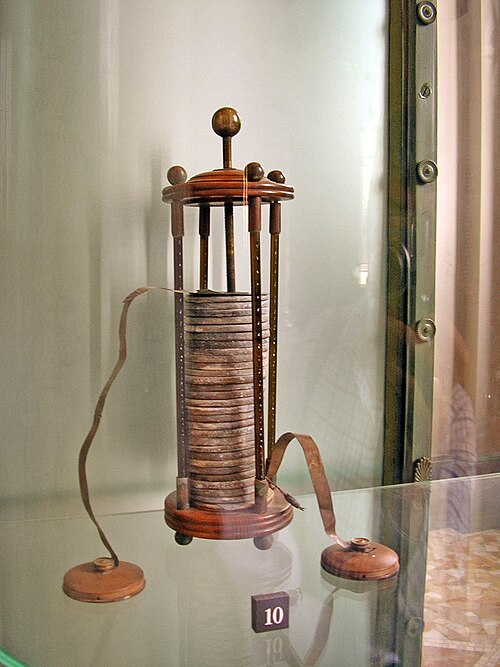
\includegraphics[width=\linewidth]{images/book3/volta-pile.jpg}
\end{minipage}\hfill
\begin{minipage}[t]{0.69\linewidth}
\vspace{0pt}
وصف أليساندرو فولتا سنة 1800 عمودًا من أقراص من فلزين مختلفين،
الزنك والنحاس أو الفضة، تفصل بينها قطع قماش مبللة بماء مالح: وكان أول
مصدر لتيار كهربائي مستمر. وفي غضون أسابيع استعمله آخرون في تفكيك
الماء، وفي غضون عقد كان همفري ديفي قد عزل الصوديوم والبوتاسيوم \omterm{def:b2:batteries-electrolysis:electrolysis}{بالتحليل
الكهربائي} لهيدروكسيديهما المنصهرين بعمود كبير. وتُظهر الصورة
أحد أعمدة فولتا نفسه. (صورة: غيدوب، CC~BY-SA~3.0، ويكيميديا
كومنز.)
\end{minipage}
\end{history}

\section{خلايا الوقود}

\begin{definition}[خلية الوقود]\label{def:b2:batteries-electrolysis:fuel-cell}
\emph{خلية الوقود}\index{خلية وقود} خلية تُغذّى كواشفها، أي وقود
ومؤكسد (هو عادة أكسجين الهواء)، باستمرار إلى
قطبيها وتُزال نواتجها، بحيث تعطي تيارًا ما دامت
تُمَدّ.
\end{definition}

في خلية غشاء التبادل البروتوني في حافلة
\cref{ch:b2:cell-thermodynamics}، يتأكسد الهيدروجين على حفاز من البلاتين،
\ce{H2 -> 2H+ + 2e-}، وتعبر البروتونات غشاءً بوليميريًا حمضيًا رقيقًا، ويُختزل الأكسجين
على الجانب الآخر، \ce{O2 + 4H+ + 4e- -> 2H2O}. وأكسدة الهيدروجين
على البلاتين \omterm{def:b2:current-potential-curves:fast-slow}{نظام سريع}؛ أما اختزال الأكسجين فبطيء على كل
قطب. ومعظم الجهد المفقود بين \qty{1.23}{V} للخلية
العكوسة وجهد التشغيل هو \omterm{def:b2:current-potential-curves:overpotential}{فرط جهد} قطب الأكسجين،
والباقي مقاومة الغشاء، وعند التيار المرتفع، إمداد الحفاز
بالأكسجين (\omterm{def:b2:current-potential-curves:limiting-current}{تيار حدي}).

\section{التحليل الكهربائي}

\begin{definition}[التحليل الكهربائي]\label{def:b2:batteries-electrolysis:electrolysis}
\emph{التحليل الكهربائي}\index{تحليل كهربائي} تفاعل أكسدة واختزال غير تلقائي
يفرضه تيار يمده مولّد خارجي؛ والخلية التي يجري فيها
هي \emph{جهاز التحليل الكهربائي}\index{جهاز تحليل كهربائي}. والمصعد، حيث تجري
الأكسدة، موصول بالقطب الموجب للمولّد.
\end{definition}

\begin{proposition}[الجهد الأدنى الترموديناميكي]\label{prop:b2:batteries-electrolysis:minimum-voltage}
\omterm{def:b2:batteries-electrolysis:electrolysis}{التحليل الكهربائي} الذي لتفاعله $\Delta_r G > 0$ يتطلب جهدًا لا يقل
عن $\Delta_r G/(nF)$.
\end{proposition}

\begin{proof}
يمد المولّد الشغل $nFU$ لكل مول من التفاعل؛ وحسب
\cref{thm:b2:cell-thermodynamics:delta-g-nfe} مطبَّقةً على التفاعل المعاكس، يجب ألا يقل
الشغل الكهربائي المستقبَل عن $\Delta_r G$.
\end{proof}

\begin{proposition}[جهد جهاز التحليل الكهربائي]\label{prop:b2:batteries-electrolysis:electrolysis-voltage}
يحتاج \omterm{def:b2:batteries-electrolysis:electrolysis}{جهاز تحليل كهربائي} يمرر تيارًا $I$ إلى
\[
  U = (E_a - E_c) + \eta_a + |\eta_c| + rI ,
\]
حيث $E_a$ و$E_c$ جهدا التوازن لمزدوجتي المصعد والمهبط
($E_a - E_c = \Delta_r G/(nF)$)، و$\eta_a$ و$\eta_c$ فرطا جهدهما عند ذلك
التيار، و$r$ المقاومة بين القطبين.
\end{proposition}

\begin{proof}
كما في الخلية، التيار نفسه مصعدي عند المصعد، عند الجهد $E_a +
\eta_a$، ومهبطي عند المهبط، عند $E_c + \eta_c$؛ ويجب على المولّد أيضًا
أن يدفعه عبر الإلكتروليت، فيضيف $rI$.
\end{proof}

\begin{method}[التنبؤ بنتيجة تحليل كهربائي]\label{met:b2:batteries-electrolysis:predict-electrolysis}
\begin{enumerate}
  \item اذكر كل الأنواع التي يمكن أن تتأكسد عند المصعد (ومنها
        فلز المصعد والمذيب) وكل الأنواع التي يمكن أن تُختزل عند
        المهبط (ومنها المذيب).
  \item ارسم منحنيات شدة التيار--الجهد لها على مواد الأقطاب المستعملة.
  \item كلما رُفع الجهد، فإن أول منحنى مصعدي وأول منحنى مهبطي
        يُبلغان يعطيان التفاعلين؛ وعند تيارات أكبر تضيف المنحنيات التالية
        تفاعلاتها.
\end{enumerate}
\end{method}

\begin{definition}[المردود الفارادي]\label{def:b2:batteries-electrolysis:faradaic-efficiency}
\emph{المردود الفارادي}\index{مردود فارادي} $\eta_F$ \omterm{def:b2:batteries-electrolysis:electrolysis}{لتحليل
كهربائي} هو كسر الشحنة المارة الذي ينتج الناتج
المطلوب. و\emph{الاستهلاك النوعي للطاقة}\index{استهلاك نوعي للطاقة}
هو الطاقة الكهربائية المستعملة لكل وحدة كتلة من الناتج.
\end{definition}

\begin{proposition}[قانون فاراداي]\label{prop:b2:batteries-electrolysis:faraday-mass}
التيار $I$ المار مدة $t$ \omterm{def:b2:batteries-electrolysis:faradaic-efficiency}{بمردود فارادي} $\eta_F$ ينتج
كتلة $m = \eta_F MIt/(nF)$ من ناتج كتلته المولية $M$ يتكوّن مع $n$
إلكترونًا لكل مول.
\end{proposition}

\begin{proof}
الشحنة $It$، التي يكوّن جزؤها $\eta_F It$ الناتج، توافق حسب
\cref{prop:b2:cell-thermodynamics:charge} $\eta_F It/(nF)$ مولًا.
\end{proof}

\begin{proposition}[الطاقة لكل كيلوغرام]\label{prop:b2:batteries-electrolysis:energy}
عند جهد $U$ \omterm{def:b2:batteries-electrolysis:faradaic-efficiency}{ومردود فارادي} $\eta_F$، يكون \omterm{def:b2:batteries-electrolysis:faradaic-efficiency}{الاستهلاك النوعي
للطاقة} $w = nFU/(\eta_F M)$.
\end{proposition}

\begin{proof}
الطاقة $UIt$ والكتلة $\eta_F MIt/(nF)$؛ نقسم.
\end{proof}

\section{عمليات التحليل الكهربائي الصناعية}

\paragraph{الزنك.} يُستخلص أغلب الزنك \omterm{def:b2:batteries-electrolysis:electrolysis}{بالتحليل الكهربائي} لمحلول كبريتات الزنك
الحمضي الوارد في \cref{ch:b2:ellingham}. ويترسب الزنك على المهبط مع أن
\ce{H+} هو المؤكسد الأقوى: فاختزال \ce{H+} على الزنك بطيء جدًا،
وتُبلغ موجة الزنك أولًا؛ ويطلق المصعد الأكسجين.

\begin{omfigure}
\begin{tikzpicture}
\begin{axis}[omie, width=0.82\linewidth, height=5.6cm, xmin=-1.6, xmax=2.4,
  ymin=-2.4, ymax=2.4, xlabel={\babelsublr{$E$ (V)}}, ylabel={$i$}, clip=true, clip mode=individual]
\addplot[omcathodic] table[x=E, y=i] {figdata/out/bachelor-2-ie-curves-g-cath.dat};
\addplot[omanodic] table[x=E, y=i] {figdata/out/bachelor-2-ie-curves-g-an.dat};
\draw[densely dotted] (axis cs:-0.76,-2.2) -- (axis cs:-0.76,0.4);
\draw[densely dotted] (axis cs:0,-2.2) -- (axis cs:0,0.4);
\node[font=\scriptsize, anchor=south] at (axis cs:-0.76,0.4) {$-0.76$};
\node[font=\scriptsize, anchor=south east] at (axis cs:-0.02,0.4) {$0$};
\node[font=\scriptsize, omDef, anchor=north west, align=left] at (axis cs:-0.7,-1.05) {\babelsublr{\ce{Zn^2+} $\to$ \ce{Zn}}،\\ استواء};
\node[font=\scriptsize, omDef, anchor=east, align=right] at (axis cs:-1.32,-0.9) {\babelsublr{\ce{H+} $\to$ \ce{H2}}\\ \foreignlanguage{arabic}{على \babelsublr{Zn}}};
\node[font=\scriptsize, omThm, anchor=east] at (axis cs:1.85,1.6) {\babelsublr{\ce{H2O} $\to$ \ce{O2}}};
\node[font=\scriptsize, gray, align=center] at (axis cs:-0.38,-0.5) {\foreignlanguage{arabic}{لا \ce{H2}}\\ على الزنك هنا};
\end{axis}
\end{tikzpicture}

{\small \omterm{def:b2:batteries-electrolysis:electrolysis}{التحليل الكهربائي} لمحلول حمضي من كبريتات الزنك بمهبط من الزنك
(منحنيات نموذجية). مع أن المزدوجة $\ce{H+}/\ce{H2}$ ($\qty{0}{V}$) تقع فوق
$\ce{Zn^2+}/\ce{Zn}$ ($\qty{-0.76}{V}$)، فإن اختزال \ce{H+} على الزنك لا
يبدأ قبل نحو \qty{-1.1}{V}: وبينهما يترسب الزنك وحده. وعند
المصعد يتأكسد الماء إلى أكسجين.}
\end{omfigure}

\paragraph{الكلور وهيدروكسيد الصوديوم.} يُحلَّل الماء المالح كهربائيًا في خلية
يقسمها غشاء لا يسمح إلا بمرور الكاتيونات. عند المصعد يتأكسد الكلوريد،
\ce{2Cl- -> Cl2 + 2e-}؛ وعند المهبط يُختزل الماء، \ce{2H2O +
2e- -> H2 + 2OH-}؛ وتعبر أيونات الصوديوم الغشاء لموازنة الشحنة، ويخرج
محلول هيدروكسيد الصوديوم من جهة المهبط، خاليًا من الكلوريد. والحد
الأدنى الترموديناميكي $\Delta_r G/(2F) = \qty{2.19}{V}$ للتفاعل \ce{2Cl- + 2H2O -> Cl2 +
H2 + 2OH-} في الشروط القياسية. ويتكوّن الكلور عند المصعد بدل
الأكسجين، مع أن المزدوجة $\ce{O2}/\ce{H2O}$ تقع أدنى: فأكسدة الماء
هي الأبطأ بين الاثنتين على مواد المصاعد المستعملة.
% ledger: dfg:OH-_ao, dfg:Cl-_ao, dfg:H2O_l

\begin{omfigure}
\begin{tikzpicture}[font=\small, >={Stealth}]
  \draw[thick] (0,0) rectangle (6,3.4);
  \draw[thick, dashed, omProp] (3,0) -- (3,3.4);
  \fill[black!30] (0.4,0.3) rectangle (0.7,3.0);
  \fill[black!50] (5.3,0.3) rectangle (5.6,3.0);
  \node[font=\scriptsize] at (0.55,3.3) {$+$};
  \node[font=\scriptsize] at (5.45,3.3) {$-$};
  \node[font=\scriptsize, align=center] at (1.85,1.9) {ماء مالح\\ \babelsublr{\ce{2Cl-} $\to$}\\ \ce{Cl2 + 2e-}};
  \node[font=\scriptsize, align=center] at (4.2,1.9) {\foreignlanguage{arabic}{محلول}\\ \ce{NaOH}\\ \babelsublr{\ce{2H2O + 2e-} $\to$}\\ \ce{H2 + 2OH-}};
  \draw[->, thick, omDef] (2.6,0.8) -- (3.4,0.8) node[pos=0.1, above, font=\scriptsize] {\ce{Na+}};
  \draw[->, thick] (1.0,3.4) -- (1.0,4.0) node[above] {\ce{Cl2}};
  \draw[->, thick] (5.0,3.4) -- (5.0,4.0) node[above] {\ce{H2}};
  \draw[->, thick] (-0.8,0.6) -- (0,0.6) node[pos=0, left] {دخول الماء المالح};
  \draw[->, thick] (6,0.6) -- (6.8,0.6) node[right] {\foreignlanguage{arabic}{خروج \ce{NaOH}}};
  \node[font=\scriptsize, omProp, anchor=north] at (3,-0.05) {غشاء تبادل كاتيوني};
\end{tikzpicture}

{\small خلية كلور--قلوي غشائية، رسم تخطيطي. لا تعبر الغشاءَ إلا أيونات
الصوديوم، فلا يلاقي الهيدروكسيدُ المتكوّن عند المهبط الكلورَ.}
\end{omfigure}

\paragraph{الألومنيوم.} يُذاب أكسيد الألومنيوم في الكريوليت المنصهر،
\ce{Na3AlF6}، الذي ينصهر عند درجة أدنى بكثير من الألومينا، ويُحلَّل كهربائيًا بين
مهبط من الكربون، يتجمع عليه الألومنيوم السائل، ومصاعد من الكربون
تحترق على هيئة ثنائي أكسيد الكربون (طريقة هول--هيرو):
\[
  \ce{2Al2O3 + 3C -> 4Al + 3CO2} .
\]
الحد الأدنى الترموديناميكي قرب \qty{1250}{K} نحو \qty{1.18}{V}
(\cref{pb:b2:batteries-electrolysis:1})؛ وتعمل خلية تلك المسألة بثلاثة أضعاف
ونصف منه، ويتحول الفائض إلى الحرارة التي تُبقي الحوض
منصهرًا.

\begin{omfigure}
\begin{tikzpicture}[font=\small, >={Stealth}]
  \draw[thick, fill=black!12] (0,0) rectangle (7,3.2);
  \fill[black!45] (0.3,0.3) rectangle (6.7,0.8);
  \fill[gray!35] (0.3,0.8) rectangle (6.7,1.4);
  \fill[orange!30] (0.3,1.4) rectangle (6.7,2.5);
  \foreach \x in {1.0,3.0,5.0} {
    \fill[black!75] (\x,1.75) rectangle (\x+1.0,3.6);
    \draw[thick] (\x+0.5,3.6) -- (\x+0.5,4.2);
  }
  \draw[thick] (1.5,4.2) -- (5.5,4.2) node[right] {$+$};
  \node[font=\scriptsize, align=left, anchor=west] at (7.3,2.6) {\foreignlanguage{arabic}{مصاعد كربونية، تحترق إلى \ce{CO2}}};
  \node[font=\scriptsize, align=left, anchor=west] at (7.3,1.95) {\foreignlanguage{arabic}{كريوليت منصهر + \ce{Al2O3} مذاب}};
  \node[font=\scriptsize, align=left, anchor=west] at (7.3,1.1) {\shortstack{\foreignlanguage{arabic}{ألومنيوم سائل (مهبط)}}};
  \node[font=\scriptsize, align=left, anchor=west] at (7.3,0.55) {\foreignlanguage{arabic}{كتلة المهبط الكربونية، $-$}};
  \draw[densely dotted] (6.7,2.6) -- (7.3,2.6) (6.7,1.95) -- (7.3,1.95) (6.7,1.1) -- (7.3,1.1) (6.7,0.55) -- (7.3,0.55);
\end{tikzpicture}

{\small خلية هول--هيرو، مقطع عرضي، رسم تخطيطي. يُختزل الألومنيوم
عند سطح بركة الفلز السائل، التي تؤدي دور المهبط؛ وتتفرغ أيونات
الأكسيد على المصاعد الكربونية، فتحرقها إلى ثنائي أكسيد الكربون.}
\end{omfigure}

\begin{history}[هول وهيرو، 1886]
\begin{minipage}[t]{0.18\linewidth}
\vspace{0pt}
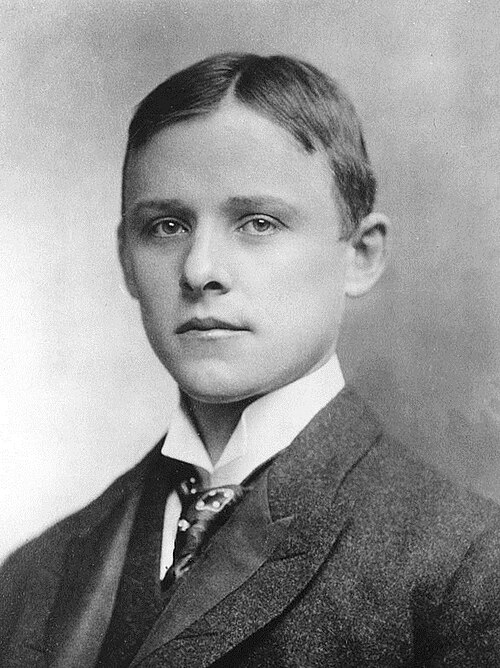
\includegraphics[width=\linewidth]{images/book3/hall.jpg}
\end{minipage}\hspace{0.02\linewidth}%
\begin{minipage}[t]{0.18\linewidth}
\vspace{0pt}
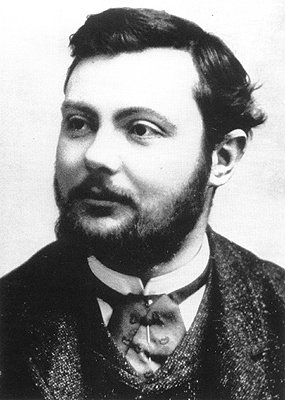
\includegraphics[width=\linewidth]{images/book3/heroult.jpg}
\end{minipage}\hfill
\begin{minipage}[t]{0.58\linewidth}
\vspace{0pt}
في سنة 1886، في الثانية أو الثالثة والعشرين من العمر، وجد تشارلز مارتن هول
وبول هيرو، على ضفتي الأطلسي، كل منهما مستقلًا عن الآخر أن الألومينا
تذوب في الكريوليت المنصهر ويمكن تحليلها كهربائيًا فيه. فصار الألومنيوم، الذي كان
حتى ذلك الحين فلزًا ثمينًا يُصنع باختزال كلوريده بالصوديوم،
أرخص الفلزات الخفيفة بمجرد أن صار توليد الكهرباء بكميات كبيرة ممكنًا.
(صورتان: هول، نحو ثمانينيات القرن التاسع عشر، مؤلف مجهول، ملكية عامة؛ هيرو،
ملكية عامة؛ ويكيميديا كومنز.)
\end{minipage}
\end{history}

\paragraph{الصوديوم.} لا يمكن ترسيب الصوديوم من الماء، الذي يختزله.
فهو يُصنع \omterm{def:b2:batteries-electrolysis:electrolysis}{بالتحليل الكهربائي} لكلوريد الصوديوم المنصهر، بعد خفض درجة انصهاره
بملح مضاف (\omterm{def:b2:solid-liquid-diagrams:eutectic}{خليط أوتكتيكي}، \cref{ch:b2:solid-liquid-diagrams})،
والكلور ناتج ثانوي. وعند \qty{1100}{K}، $\Delta_f G^\circ(\ce{NaCl}, \text{l}) =
\qty{-310.7}{kJ/mol}$: فالجهد الأدنى \qty{3.22}{V}.
% ledger: janafG:NaCl.1100

\section{تمارين}

\begin{exercise}[$\star$]\label{exo:b2:batteries-electrolysis:1}
على شكل الزنك في الحمض، اقرأ \omterm{def:b2:batteries-electrolysis:mixed-potential}{الجهد المختلط} والتيار للزنك
وحده وللزنك الملامس للنحاس (بوحدات النموذج)، وبيّن أيهما يذوب
أسرع.
\end{exercise}

\begin{exercise}[$\star$]\label{exo:b2:batteries-electrolysis:2}
ما كتلة الزنك التي يرسبها في ساعة واحدة تيار شدته \qty{500}{A} \omterm{def:b2:batteries-electrolysis:faradaic-efficiency}{بمردود
فارادي} قدره 100~\%؟
\end{exercise}

\begin{exercise}[$\star$]\label{exo:b2:batteries-electrolysis:3}
احسب الجهد القياسي \omterm{def:b2:batteries-electrolysis:battery}{لمركم} الرصاص--الحمض من طاقات جيبس
للتكوين المعطاة في الفصل، وعدد الخلايا في بطارية سيارة
جهدها \qty{12}{V}.
\end{exercise}

\begin{exercise}[$\star$]\label{exo:b2:batteries-electrolysis:4}
ما الشحنة، بالأمبير ساعي، التي يمكن أن يعطيها غرام واحد من الليثيوم إذا تأكسد
كله إلى \ce{Li+}؟
\end{exercise}

\begin{exercise}[$\star\star$]\label{exo:b2:batteries-electrolysis:5}
تمرر خلية لتنقية النحاس \qty{200}{A} مدة \qty{24}{h} وترسب
\qty{5.50}{kg} من النحاس. احسب \omterm{def:b2:batteries-electrolysis:faradaic-efficiency}{المردود الفارادي}.
\end{exercise}

\begin{exercise}[$\star\star$]\label{exo:b2:batteries-electrolysis:6}
تعمل خلية استخلاص كهربائي للزنك عند \qty{3.3}{V} \omterm{def:b2:batteries-electrolysis:faradaic-efficiency}{بمردود فارادي} قدره
90~\% (معطيات تمرين). احسب الطاقة الكهربائية لكل كيلوغرام من الزنك.
\end{exercise}

\begin{exercise}[$\star\star$]\label{exo:b2:batteries-electrolysis:7}
تعطي بطارية \qty{1.55}{V} عند \qty{0.10}{A} و\qty{1.40}{V} عند \qty{0.60}{A}.
وبافتراض \omterm{def:b2:current-potential-curves:overpotential}{فرط الجهد} مهملًا، أوجد مقاومتها الداخلية وجهدها
دون تيار.
\end{exercise}

\begin{exercise}[$\star\star$]\label{exo:b2:batteries-electrolysis:8}
يُحلَّل الماء المالح كهربائيًا في الخلية الغشائية. اكتب تفاعلات القطبين،
واحسب الجهد الأدنى، وفسّر لماذا يجب إبقاء النواتج
منفصلة.
\end{exercise}

\begin{exercise}[$\star\star$]\label{exo:b2:batteries-electrolysis:9}
احسب الجهد الأدنى \omterm{def:b2:batteries-electrolysis:electrolysis}{للتحليل الكهربائي} لكلوريد الصوديوم المنصهر عند
\qty{1100}{K} والطاقة الدنيا لكل كيلوغرام من الصوديوم.
\end{exercise}

\begin{exercise}[$\star\star\star$]\label{exo:b2:batteries-electrolysis:10}
مستعملًا منحنيات شدة التيار--الجهد، فسّر لماذا يمكن طلاء الزنك من حوض
حمضي على مهبط من الزنك، وتنبأ بما كان سيحدث على مهبط من البلاتين في
بداية الطلاء.
\end{exercise}

\begin{exercise}[$\star\star\star$]\label{exo:b2:batteries-electrolysis:11}
انطلاقًا من $\Delta_f G^\circ$ عند \qty{1100}{K} و\qty{1300}{K} ($\ce{Al2O3}$: $-1328.3$ 
و$-1262.3$؛ $\ce{CO2}$: $-396.0$ و$-396.2$ \unit{kJ/mol})، احسب الجهد
الأدنى لخلية هول--هيرو عند \qty{1250}{K}، وقارنه بمصعد خامل
يتحرر عليه الأكسجين.
\end{exercise}

\begin{exercise}[$\star\star\star$]\label{exo:b2:batteries-electrolysis:12}
تُخزَّن الكهرباء بتحليل الماء كهربائيًا عند \qty{1.80}{V} وتُسترجع في \omterm{def:b2:batteries-electrolysis:fuel-cell}{خلية
وقود} عند \qty{0.70}{V}، وكلاهما \omterm{def:b2:batteries-electrolysis:faradaic-efficiency}{بمردود فارادي} قدره 100~\%. احسب
مردود الذهاب والإياب وفسّر أين تذهب الطاقة.
\end{exercise}

\section{مسألة: طن من الألومنيوم}

\begin{problem}[{مسألة نهاية الأسبوع --- تفاعل خلية هول--هيرو
وجهدها الأدنى، والشحنة والزمن اللازمان لصنع طن من الألومنيوم،
والطاقة المستعملة، والكربون المحروق}]
\label{pb:b2:batteries-electrolysis:1}
المعطيات: طاقات جيبس للتكوين من جداول جاناف عند \qty{1100}{K} و\qty{1300}{K}
(\unit{kJ/mol}): \ce{Al2O3} $-1328.3$، $-1262.3$؛ \ce{CO2} $-396.0$، $-396.2$. الخلية
(معطيات تمرين): التيار \qty{300}{kA}، والجهد \qty{4.1}{V}، \omterm{def:b2:batteries-electrolysis:faradaic-efficiency}{والمردود الفارادي}
94~\%، والحوض قرب \qty{1250}{K}. الكتل المولية (\unit{g/mol}): Al 26.982، C 12.011،
O 15.999. الحرارة اللازمة لرفع الألومنيوم من \qty{298}{K} إلى الحالة السائلة عند
نقطة انصهاره: \qty{28.69}{kJ/mol}.
% ledger: janafG:Al2O3.1100, janafG:Al2O3.1300, janafG:CO2.1100, janafG:CO2.1300, aw:Al, aw:C, aw:O, hT:Al_l.933, const:F

\medskip
\noindent\textbf{الجزء الأول --- الجهد الأدنى.}
\begin{enumerate}
  \item أعطِ أعداد أكسدة الألومنيوم والأكسجين والكربون في
        المتفاعلات والنواتج.
  \item اكتب نصفي التفاعل عند المهبط والمصعد، مع أيون الأكسيد
        \ce{O^2-} الذي يحمله الحوض المنصهر.
  \item اكتب التفاعل الإجمالي وعدد الإلكترونات المتبادلة $n$.
  \item استوفِ $\Delta_f G^\circ$ للمركبين \ce{Al2O3} و\ce{CO2} عند \qty{1250}{K}.
  \item احسب $\Delta_r G^\circ$ عند \qty{1250}{K}.
  \item استنتج الجهد الأدنى.
  \item احسب الجهد الأدنى مع مصعد خامل،
        \ce{2Al2O3 -> 4Al + 3O2}، وفسّر دور الكربون.
\end{enumerate}

\medskip
\noindent\textbf{الجزء الثاني --- الشحنة والزمن.}
\begin{enumerate}[resume]
  \item ما كمية مادة الألومنيوم في طن واحد؟
  \item ما الشحنة التي كانت ستلزم \omterm{def:b2:batteries-electrolysis:faradaic-efficiency}{بمردود فارادي} قدره 100~\%؟
  \item ما الشحنة المارة فعلًا؟
  \item كم من الوقت تستغرق خلية واحدة لصنع طن؟
  \item ما كتلة الألومنيوم التي تصنعها خلية واحدة في اليوم؟
  \item اقترح أين تذهب نسبة 6~\% المفقودة من الشحنة.
\end{enumerate}

\medskip
\noindent\textbf{الجزء الثالث --- الطاقة.}
\begin{enumerate}[resume]
  \item احسب الطاقة الكهربائية لكل طن.
  \item عبّر عنها بوحدة \unit{kW.h} لكل كيلوغرام.
  \item احسب الطاقة الدنيا لكل كيلوغرام، عند الجهد الأدنى ومردود
        100~\%.
  \item أين تذهب بقية الطاقة، ولماذا لا تضيع
        كلها؟
  \item احسب الاستطاعة الكهربائية لخلية واحدة.
  \item احسب الحرارة اللازمة لإعادة صهر كيلوغرام من الخردة، بوحدة
        \unit{kW.h}، وقارن.
  \item ما الكسر الذي يمثله الحد الأدنى الترموديناميكي من جهد التشغيل؟
\end{enumerate}

\medskip
\noindent\textbf{الجزء الرابع --- الكربون.}
\begin{enumerate}[resume]
  \item احسب كتلة الكربون المحروق لكل طن من الألومنيوم وفق
        المعادلة.
  \item احسب كتلة ثنائي أكسيد الكربون التي تطلقها المصاعد لكل طن.
  \item تحرق الخلايا الحقيقية كربونًا أكثر من ذلك. اقترح سببين.
  \item عبّر عن \ce{CO2} الصادر عن المصاعد لكل كيلوغرام من الألومنيوم.
  \item ماذا كان سيغيّر مصعد خامل في الجهد وفي الغاز
        المتحرر؟
  \item اذكر الطاقة الكهربائية لكل كيلوغرام من الألومنيوم.
\end{enumerate}
\end{problem}
